\documentclass{beamer}
\setbeamertemplate{navigation symbols}{}

\usepackage{listings}
\lstset{basicstyle=\ttfamily}
\usepackage{tikz}
\usetikzlibrary{arrows}
\usepackage{adjustbox}

\begin{document} 

\begin{frame}{LINQ to Wiki}
\begin{itemize}
\item library for accessing MediaWiki API from .Net
\item uses LINQ for querying lists
\item strongly-typed (no magic strings)
\item the API is big, changes often and can be different for different wikis (thanks to extensions)
\begin{itemize}
\item because of that, Roslyn is used to generate code based on description the API provides about itself
\end{itemize}
\end{itemize}
\end{frame}

\begin{frame}{Modules in the API}
\begin{itemize}
\item the API is divided into modules
\item each module has a specific function
\begin{itemize}
\item examples: edit page, list all categories, show categories of a given page
\end{itemize}
\item there are three kinds of modules: simple modules, list modules and prop modules
\begin{itemize}
\item simple modules return a single result
\item list modules return a list of items as a result
\item prop modules are used to retrieve additional information about a list of pages
\begin{itemize}
\item that list can be from a list module or a hard-coded set of pages
\end{itemize}
\end{itemize}
\end{itemize}
\end{frame}

\newlength\codeheight
\setlength\codeheight{10cm}

\begin{frame}[fragile]{Simple modules}
\begin{itemize}
\item simple modules are represented as methods on the \lstinline{Wiki} class
\item parameters of modules are parameters of the method
\begin{itemize}
\item optional parameters as C\# 4 optional parameters
\item most parameters are optional
\end{itemize}
\item the result of the module is the result of the method
\end{itemize}

\medskip

\begin{adjustbox}{width=\textwidth,keepaspectratio}
\begin{lstlisting}
var wiki = new Wiki("en.wikipedia.org");

// get edit token, necessary to edit pages
var token = wiki.tokens(new[] { tokenstype.edit }).edittoken;

// create new section "Hello" on the page "Wikipedia:Sandbox"
wiki.edit(
    token: token, title: "Wikipedia:Sandbox", section: "new",
    sectiontitle: "Hello", text: "Hello world!");
\end{lstlisting}
\end{adjustbox}
\end{frame}

\begin{frame}{List modules}
\begin{itemize}
\item list modules are methods on the \lstinline{Query} property of \lstinline{Wiki}
\item query can be modified by using LINQ methods \lstinline{Where()}, \lstinline{OrderBy()} (where available) and \lstinline{Select()}
\begin{itemize}
\item different properties can be used for each method
\begin{itemize}
\item example: pages can't be ordered or filtered by their text, but the text can be selected
\end{itemize}
\item query syntax (\lstinline{from}, \lstinline{where}, \lstinline{orderby} and \lstinline{select}) can be used instead of method syntax
\item other LINQ methods (or query operators) can't be used (won't compile)
\item lambdas are compiled as expressions, parsed into API parameters
\item \lstinline{Select()} lambda can contain any code, \lstinline{Where()} and \lstinline{OrderBy()} can't
\end{itemize}
\item each query ends by a call to \lstinline{ToEnumerable()} or \lstinline{ToList()}
\end{itemize}
\end{frame}

\begin{frame}[fragile]{List modules example}
\begin{adjustbox}{width=\textwidth,keepaspectratio}
\begin{lstlisting}
var pages = (from cm in wiki.Query.categorymembers()
             where cm.title == "Category:Query languages"
             orderby cm.sortkey descending
             select cm.title)
            .ToEnumerable();
\end{lstlisting}
\end{adjustbox}

\medskip

\begin{itemize}
\item \lstinline{pages} is a lazy list of page titles (\lstinline{IEnumerable<string>}) in the category ``Query languages'', sorted by their ``sortkey'' in reverse
\begin{itemize}
\item the laziness means that for example enumerating \lstinline{pages.Take(10)} will only make one request, for the first page of results
\end{itemize}
\end{itemize}
\end{frame}

\begin{frame}[fragile]{Page sources}
\begin{itemize}
\item prop modules work on page sources (\lstinline{PagesSource})
\item page source can be created from a static list of pages:
\end{itemize}
\begin{adjustbox}{scale=0.7}
\begin{lstlisting}
    var source = wiki.CreateTitlesSource("C Sharp", "LINQ");
\end{lstlisting}
\end{adjustbox}
\begin{itemize}
\item or they can be created from some queries without a \lstinline{Select()}
by accessing the \lstinline{Pages} property:
\end{itemize}
\begin{adjustbox}{scale=0.7}
\begin{lstlisting}
    var source = (from cm in wiki.Query.categorymembers()
                  where cm.title == "Category:Query languages"
                  select cm)
                 .Pages;
\end{lstlisting}
\end{adjustbox}
\begin{itemize}
\item[]
\begin{itemize}
\item \lstinline{select cm} here doesn't result in a \lstinline{Select()} call
\end{itemize}
\end{itemize}
\end{frame}

\begin{frame}{Prop modules}
\begin{itemize}
\item given a page source, you can use \lstinline{Select()} to access one or more prop modules
\item the lambda parameter has a member for each prop module
\begin{itemize}
\item prop modules that return lists are methods, whose result can be used with LINQ methods
\item \lstinline{ToEnumerable()} (or \lstinline{ToList()}) has to be called at the end of each subquery
\item prop modules that return single result are properties
\end{itemize}
\item the lambda can contain arbitrary code, except for the part of each subquery before \lstinline{ToEnumerable()}
\item it doesn't matter whether the page source is from another query or from a static list
\end{itemize}
\end{frame}

\begin{frame}[fragile]{Prop modules example}

\begin{adjustbox}{width=\textwidth,keepaspectratio}
\begin{lstlisting}
var pages = source
    .Select(
        p =>
        new
        {
            p.info,
            categories =
            p.categories()
                .Where(c => c.show == categoriesshow.not_hidden)
                .Select(c => new { c.title, c.sortkeyprefix })
                .ToEnumerable()
                .Take(1)
        }
    ).ToEnumerable();
\end{lstlisting}
\end{adjustbox}
\begin{itemize}
\item \lstinline{pages} is a lazy collection of anonymous objects, each containing the basic information about a page, along with \lstinline{title} and \lstinline{sortkeyprefix} of the first category of that page that is not hidden
\end{itemize}
\end{frame}

\begin{frame}{Code generation}
\begin{itemize}
\item the \texttt{linqtowiki-codegen} console application can be used to generate assembly for a given wiki
\item it should be run again when the API changes or for working with different wiki
\item but if the changes are not relevant, the generated assembly for an older version or for different wiki can be used
\item the code can be generated into a specified namespace, so that assemblies for different wikis could be used from one application
\item the application requires Roslyn
\end{itemize}
\end{frame}

\begin{frame}{LINQ implementation}
\begin{itemize}
\item the desired behavior of LINQ methods is achieved by a group of types whose names start with \lstinline{WikiQuery}
\item each type defines the members it can support
\item invoking a member stores the changes it made and can return a different type
\end{itemize}

\begin{center}
\begin{adjustbox}{scale=.5}
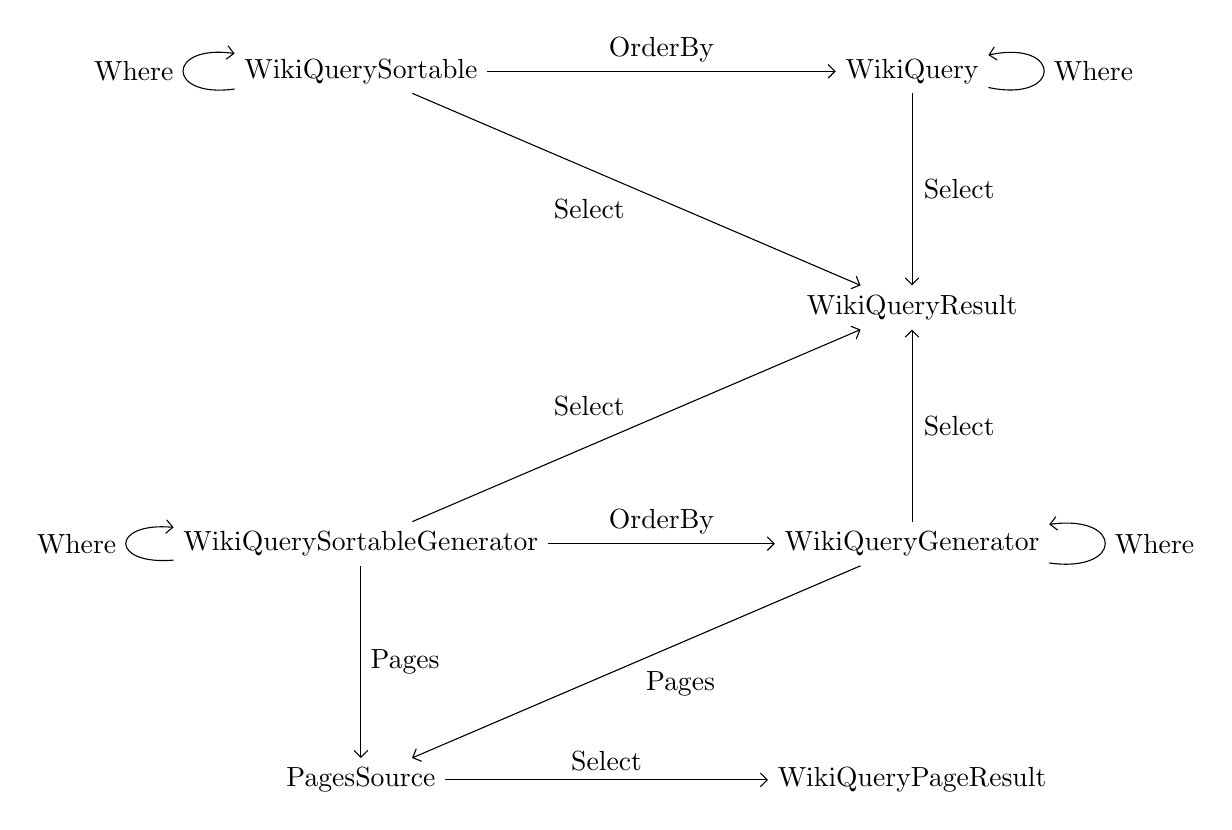
\begin{tikzpicture}[>=angle 90]
\path (-2,9) node(WQS) {\lstinline{WikiQuerySortable}};
\path (5,9) node(WQ) {\lstinline{WikiQuery}};

\path (5,6) node(WQR) {\lstinline{WikiQueryResult}};

\path (-2,3) node(WQSG) {\lstinline{WikiQuerySortableGenerator}};
\path (5,3) node(WQG) {\lstinline{WikiQueryGenerator}};

\path (-2,0) node(PS) {\lstinline{PagesSource}};
\path (5,0) node(WQPR) {\lstinline{WikiQueryPageResult}};

\draw[->] (WQS) edge [out=188,in=172,looseness=5,auto] node {\lstinline{Where}} (WQS);
\draw[->] (WQS) edge node[above] {\lstinline{OrderBy}} (WQ);
\draw[->] (WQS) edge node[below left] {\lstinline{Select}} (WQR);

\draw[->] (WQ) edge [out=-12,in=12,looseness=6,right] node {\lstinline{Where}} (WQ);
\draw[->] (WQ) edge node[right] {\lstinline{Select}} (WQR);

\draw[->] (WQSG) edge [out=185,in=175,looseness=5,auto] node {\lstinline{Where}} (WQSG);
\draw[->] (WQSG) edge node[auto] {\lstinline{OrderBy}} (WQG);
\draw[->] (WQSG) edge node[above left] {\lstinline{Select}} (WQR);

\draw[->] (WQG) edge [out=-8,in=8,looseness=5,right] node {\lstinline{Where}} (WQG);
\draw[->] (WQG) edge node[right] {\lstinline{Select}} (WQR);

\draw[->] (WQSG) edge node[auto] {\lstinline{Pages}} (PS);
\draw[->] (WQG) edge node[auto] {\lstinline{Pages}} (PS);

\draw[->] (PS) edge node[auto] {\lstinline{Select}} (WQPR);
\end{tikzpicture}
\end{adjustbox}
\end{center}

\end{frame}

\begin{frame}{Paging implementation}
\begin{itemize}
\item lists can have thousands or even millions results, so the API returns them in pages
\item each pages is usually 500 items (the limit is raised to 5000 for some users)
\item queries using prop modules have two kinds of paging: for the source list and for the results
\item LINQ to Wiki handles paging transparently for users
\begin{itemize}
\item in the case of static page source, the list is split into pages by LINQ to Wiki
\item otherwise, it is handled by the API and LINQ to Wiki only has to pass the correct paging parameters to the query
\end{itemize}
\item \lstinline{ToEnumerable()} returns a lazy collection, which means only the necessary pages are retrieved
\item in prop modules queries, both kinds of paging can be lazy independently
\end{itemize}
\end{frame}

\begin{frame}{Codegen implementation}
\begin{itemize}
\item information about modules necessary to generate the code is returned by the \texttt{paraminfo} module
\begin{itemize}
\item LINQ to Wiki is used internally to access this module, although with the part that is usually generated written manually
\end{itemize}
\item the module returns description of parameters and result properties of modules
\begin{itemize}
\item the types of parameters or properties can be either simple types (e.g. string, integer) or enumerated types
\item some enumerated types can be combined together and they can also have more than 64 values, so they are not generated as \lstinline{enum}s (because they couldn't be flag enums)
\item some properties have more complex types, these are not represented in \lstinline{paraminfo}, so they aren't present in LINQ to Wiki either
\end{itemize}
\item Roslyn is used to generate the code through a helper class that makes the code simpler
\item CodeDOM is used to actually compile the generated code, because Roslyn compiler does not support all features of C\# yet (like object initializers)
\end{itemize}
\end{frame}

\begin{frame}{Codegen implementation}
\begin{itemize}
\item the following types are always generated: \lstinline{Wiki} for simple modules, \lstinline{Query} for list modules and \lstinline{Page} for prop modules
\item for each simple module, its result type is also generated
\item for each list modules, \lstinline{Where}, \lstinline{Select} and possibly \lstinline{OrderBy} type is generated
\item prop modules behave as simple modules or list modules in this regard, depending on whether they return single item or a list
\item a type is also generated for each enumerated type that is used by a parameter or a property
\end{itemize}
\end{frame}

\end{document}

\begin{itemize}
\end{itemize}